         \chapter{Physical and chemical change}\fancyfoot[LO,RE]{Chemistry: Chemical change}
    \setcounter{figure}{1}
    \setcounter{subfigure}{1}
    \label{m38709*cid1}
            \section{Introduction}
            \nopagebreak
            \label{m38709} $ \hspace{-5pt}\begin{array}{cccccccccccc}   \end{array} $ \hspace{2 pt}\raisebox{-5 pt}{
\includegraphics[width=0.5cm]{col11305.imgs/summary_www.png}} {(section shortcode: P10056 )} \par 
      \label{m38709*id62175}Matter is all around us. The desks we sit at, the air we breathe and the water we drink are all examples of matter. But matter doesn't always stay the same. It can change in many different ways. In this chapter, we are going to take a closer look at \textbf{physical} and \textbf{chemical} changes that occur in matter.\par 
    \label{m38709*cid2}
            \subsection*{Physical changes in matter}
            \nopagebreak
      \label{m38709*id62200}A \textbf{physical change} is one where the particles of the substances that are involved in the change are not broken up in any way. When water is heated for example, the temperature and energy of the water molecules increases and the liquid water evaporates to form water vapour. When this happens, some kind of change has taken place, but the molecular structure of the water has not changed. This is an example of a \textsl{physical change}. All changes in state are physical changes.\par 
      \label{m38709*id62556}$\text{H}_{2}\text{O (}\ell \text{)} \to \text{H}_{2}\text{O (g)}$
      \par 
      \label{m38709*id62600}Conduction (the transfer of energy through a material) is another example of a physical change. As energy is transferred from one material to another, the \textsl{energy} of each material is changed, but not its chemical makeup. Dissolving one substance in another is also a physical change.\par 

\label{m38709*fhsst!!!underscore!!!id76} 
 \Definition{ Physical change } { A change that can be seen or felt, but that doesn't involve the break up of the particles in the reaction. During a physical change, the \textsl{form} of matter may change, but not its \textsl{identity}. } 

      \label{m38709*id62640}There are some important things to remember about physical changes in matter:\par 
      \label{m38709*id62644}\begin{enumerate}[noitemsep, label=\textbf{\arabic*}. ] 
            \label{m38709*uid1}\item \textsl{Arrangement of particles}\newline
When a physical change occurs, the compounds may re-arrange themselves, but the bonds in between the atoms will not break. For example when liquid water boils, the molecules will move apart but the molecule will stay intact. In other words water will not break up into hydrogen and oxygen atoms.

Figure~\ref{fig:physical change:water phases} shows this phase change. Note that the water molecules themselves stay the same, but their arrangement changed.
    \setcounter{subfigure}{0}
	\begin{figure}[H] % horizontal\label{m38709*uid2}
\begin{figure}[h]
\begin{center}
\begin{pspicture}(0,0)(10,2.6)
\SpecialCoor
%\psgrid[gridcolor=lightgray]
\def\water{\psset{unit=0.25}\rput{150}{\pscircle(0,0){2}
\psarc[fillcolor=white,fillstyle=solid](-1.5,1){1.5}{30}{260}
\psarc[fillcolor=white,fillstyle=solid](1.5,1){1.5}{280}{150}
\rput(-1.5,1){\pscurve(1.5;30)(-1;142.5)(1.5;260)}
\rput(1.5,1){\pscurve(1.5;150)(-1;37.5)(1.5;280)}}}

\rput(2,0){\psframe(0,0.5)(3,2.5)
\rput(1.5,1){\psset{unit=0.5}\rput(-0.7,-0.2){\water}
\rput{185}(-1,0.9){\water}
\rput{120}(2,0.6){\water}
\rput{310}(-2.1,0){\water}
\rput{60}(0.6,1.1){\water}
\rput(1.2,-0.2){\water}}}

\rput(5,0){\psframe(0,0.5)(3,2.5)
\rput(1.5,1){\psset{unit=0.5}\rput{120}(2,1){\water}
\rput{250}(-1,2){\water}
\rput{70}(0,.5){\water}
\rput{150}(-1.5,-.2){\water}}}

\uput[d](3,0.5){liquid}
\uput[d](6,0.5){gas}

\end{pspicture}
\end{center}
\caption{The arrangement of water molecules in the liquid and gas phase}
\label{fig:physical change:water phases}
\end{figure}
 \end{figure}   
\IFact{The bonding of hydrogen and oxygen to form water is explosive and if the water molecule broke apart everytime water boiled, life on Earth would not exist for very long!}    
\label{m38709*uid221}\item \textsl{Conservation of mass}\newline
    In a physical change, the total mass, the number of atoms and the number of molecules will always stay the same. In other words you will always have the same number of molecules or atoms at the end of the change as you had at the beginning. 
\label{m38709*uid3}\item \textsl{Energy changes}\newline
Energy changes may take place when there is a physical change in matter, but these energy changes are normally smaller than the energy changes that take place during a chemical change.
\label{m38709*uid4}\item \textsl{Reversibility}\newline
Physical changes in matter are usually easier to reverse than chemical changes. Methods such as filtration and distillation can be used to reverse the change. Changing the temperature is another way to reverse a physical change. For example, a mixture of salt and water can be seperated by filtration, ice can be changed to liquid water and back again by changing the temperature.
\end{enumerate}
        \label{m38709*eip-904}\begin{activity}{Physical change}Use plastic pellets or marbles to represent water in the solid state. What do you need to do to the pellets to represent the change from solid to liquid? \\
Make a mixture of sand and water. Filter this mixture. What do you observe? \\
Make a mixture of iron filings and sulfur. Can you seperate the mixture with a magnet?  
\end{activity}
\nopagebreak
\label{m38709*secfhsst!!!underscore!!!id243}
            \begin{g_experiment}{The synthesis of iron sulphide }
            \nopagebreak
            \label{m38709*id63437}\noindent{}\textbf{Aim:} \\
     To demonstrate the synthesis of iron sulphide from iron and sulphur. \\
        \label{m38709*id63447}\noindent{}\textbf{Apparatus:} \\
$5,6~\text{g}$ iron filings and $3,2~\text{g}$ powdered sulphur; porcelain dish; test tube; Bunsen burner \\
        \label{m38709*id63457}
    \setcounter{subfigure}{0}
% 	\begin{figure}[H] % horizontal\label{m38709*id63460}
    \begin{center}
\scalebox{.6}{
\begin{pspicture}(0,0)(5,5)
\psset{unit=0.5cm,tubeSeul=true,pince=true}
\newpsstyle{gray} {linestyle=none,fillstyle=solid,fillcolor=darkgray}
\newpsstyle{orange} {linestyle=none,fillstyle=solid,fillcolor=orange}
%playing with colours, try tweak this to look like the real thing, add photo of the real thing?
\pstChauffageTube[aspectLiquide1=gray,aspectLiquide2=orange,niveauLiquide1=40,niveauLiquide2=20]
\end{pspicture}
}
    \end{center}
%  \end{figure}        
        \label{m38709*id63467}\noindent{}\textbf{Method:} 
        \label{m38709*id63473}\begin{enumerate}[noitemsep, label=\textbf{\arabic*}. ] 
            \label{m38709*uid20}\item 
Measure the quantity of iron and sulphur that you need and mix them in a porcelain dish.
\label{m38709*uid21}\item 
Take some of this mixture and place it in the test tube. The test tube should be about one third full.
\label{m38709*uid22}\item 
Heat the test tube containing the mixture over the Bunsen burner. Increase the heat if no reaction takes place. Once the reaction begins, you will need to remove the test tube from the flame. Record your observations.
\label{m38709*uid23}\item
 Wait for the product to cool before breaking the test tube with a hammer. Make sure that the test tube is rolled in paper before you do this, otherwise the glass will shatter everywhere and you may be hurt.
\label{m38709*uid24}\item 
What does the product look like? Does it look anything like the original reactants? Does it have any of the properties of the reactants (e.g. the magnetism of iron)?
\end{enumerate}
        \label{m38709*eip-963}
      \Warning{When working with a bunsen burner work in a well ventilated space and ensure that there are no flammable substances close by. Always tuck loose clothing in and ensure that long hair is tied back.}
      \label{m38709*id63554}\noindent{}\textbf{Results:} 
After you removed the test tube from the flame, the mixture glowed a bright red colour. The reaction is exothermic and \textsl{produces heats}. The product, iron sulphide, is a dark colour and does not share any of the properties of the original reactants. It is an entirely new product.\\
        \label{m38709*id63594}\noindent{}\textbf{Conclusions:} \\
A synthesis reaction has taken place. The equation for the reaction is:
        \label{m38709*id63604}\nopagebreak\noindent{}
    \begin{equation*}
    \text{Fe (s)}+\text{S (s)}\to \text{FeS (s)}
      \end{equation*} 
\end{g_experiment}
    \label{m38709*cid3}
            \subsection*{Chemical Changes in Matter}
            \nopagebreak
      \label{m38709*id62778}When a \textbf{chemical change} takes place, new substances are formed in a chemical reaction. These new products may have very different properties from the substances that were there at the start of the reaction.\par 
            \label{m38709*fhsst!!!underscore!!!id107}
 \Definition{Chemical change } { \label{m38709*meaningfhsst!!!underscore!!!id107}
      The formation of new substances in a chemical reaction. One type of matter is changed into something different. 
       } 
We will consider two examples of chemical change: the decomposition (breaking down) of hydrogen peroxide and the synthesis (forming) of water. \\
\subsubsection*{Decomposition of hydrogen peroxide}
      \label{m38709*id62788}The decomposition (breakdown) of hydrogen peroxide ($\text{H}_{2}\text{O}_{2}$) to form water ($\text{H}_{2}\text{O}$) and oxygen gas ($\text{O}_{2}$) is an example of chemical change. A simplified diagram of this reaction is shown in Figure~\ref{fig:chemical change:decomposition}. The chemical bonds between $\text{O}$ and $\text{H}$ in $\text{H}_{2}\text{O}_{2}$ are broken and new bonds between $\text{H}$ and $\text{O}$ (to form $\text{H}_{2}\text{O}$) and between $\text{O}$ and $\text{O}$ (to form $\text{O}_{2}$) are formed. A chemical change has taken place.\par 
    \setcounter{subfigure}{0}
\begin{figure}[h]
\begin{center}
\scalebox{.8}{
\begin{pspicture}(-6,-1.5)(12,1.5)
%\psgrid[gridcolor=lightgray]
%reactants
\rput(-2,0){
\psellipse(-3,0)(0.5,0.5)
\rput(-3,0){$\text{O}$}
\psellipse(-2,0)(0.5,0.5)
\rput(-2,0){$\text{O}$}
\psellipse(-3.3,-0.75)(0.3,0.3)
\rput(-3.3,-0.75){$\text{H}$}
\psellipse(-1.7,0.75)(0.3,0.3)
\rput(-1.7,0.75){$\text{H}$}
\rput(3,0){
\psellipse(-3,0)(0.5,0.5)
\rput(-3,0){$\text{O}$}
\psellipse(-2,0)(0.5,0.5)
\rput(-2,0){$\text{O}$}
\psellipse(-3.3,-0.75)(0.3,0.3)
\rput(-3.3,-0.75){$\text{H}$}
\psellipse(-1.7,0.75)(0.3,0.3)
\rput(-1.7,0.75){$\text{H}$}
}
%products
\psline[arrows=->](2,0)(4,0)
\psellipse(5,0)(0.5,0.5)
\rput(5,0){$\text{O}$}
\psellipse(4.5,0.65)(0.3,0.3)
\rput(4.5,0.65){$\text{H}$}
\psellipse(5.5,0.65)(0.3,0.3)
\rput(5.5,0.65){$\text{H}$}
\rput(2,-0.5){
\psellipse(5,0)(0.5,0.5)
\rput(5,0){$\text{O}$}
\psellipse(4.5,0.65)(0.3,0.3)
\rput(4.5,0.65){$\text{H}$}
\psellipse(5.5,0.65)(0.3,0.3)
\rput(5.5,0.65){$\text{H}$}
}
\rput(8.5,0){\textbf{+}}
\psellipse(9.5,0)(0.5,0.5)
\rput(9.5,0){$\text{O}$}
\psellipse(10.5,0)(0.5,0.5)
\rput(10.5,0){$\text{O}$}
}
\end{pspicture}
}
\end{center}
\caption{The decomposition of $\text{H}_{2}\text{O}_{2}$ to form $\text{H}_{2}\text{O}$ and $\text{O}_{2}$}
\label{fig:chemical change:decomposition}
\end{figure}     
\par
\label{m38709*secfhsst!!!underscore!!!id163}
            \begin{g_experiment}{The decomposition of hydrogen peroxide}
            \nopagebreak
            \label{m38709*id63175}\noindent{}\textbf{Aim:}\newline
    To observe the decomposition of hydrogen peroxide when it is heated.\par 
        \label{m38709*id63194}\noindent{}\textbf{Apparatus:}\newline
    Dilute hydrogen peroxide (about 3\%); manganese dioxide; test tubes; a water bowl; stopper and delivery tube, bunsen burner\par 
        \label{m38709*eip-470}
\Warning{Hydrogen peroxide can cause chemical burns. Work carefully with it.}
	\par
      \label{m38709*id63199}
    \setcounter{subfigure}{0}
	\begin{figure}[H] % horizontal\label{m38709*id63200}
    \begin{center}
\scalebox{0.8}{
\begin{pspicture}(0,0)(5,5)
\psset{unit=0.5cm,glassType=erlen,recuperationGaz,niveauLiquide1=20}
\pstChauffageBallon[tubeRecourbe]
\end{pspicture}
}
    \end{center}
 \end{figure}       
        \par 
        \label{m38709*id63206}\noindent{}\textbf{Method:}\label{m38709*id63212}\begin{enumerate}[noitemsep, label=\textbf{\arabic*}. ] 
            \label{m38709*uid11}\item Put a small amount (about $5~\text{ml}$) of hydrogen peroxide in a test tube.
\label{m38709*uid12}\item Set up the apparatus as shown above.
\label{m38709*uid13}\item Very carefully add a small amount (about $0,5~\text{g}$) of manganese dioxide to the test tube containing hydrogen peroxide. 
\end{enumerate}
        \par 
        \label{m38709*id63254}\noindent{}\textbf{Results:}\newline
    You should observe a gas bubbling up into the second test tube. This reaction happens quite rapidly. \par 
        \label{m38709*id63302}\noindent{}\textbf{Conclusions:}\newline
    When hydrogen peroxide is added to manganese dioxide it decomposes to form oxygen and water. The chemical decomposition reaction that takes place can be written as follows:
        \label{m38709*id63313}\nopagebreak\noindent{}
    \begin{equation*}
    2{\text{H}}_{2}{\text{O}}_{2} \text{(aq)} \to 2\text{H}_{2}\text{O}(\ell) + {\text{O}}_{2}\text{(g)}
      \end{equation*}
Note that the manganese dioxide is a catalyst and is not shown in the reaction. (A catalyst helps speed up a chemical reaction.)    \par 
\end{g_experiment}
\label{m38709*eip-619}
\Note{This experiment used the downward displacement of water to collect a gas. This is a very common way to collect a gas in chemistry. The oxygen that is evolved in this reaction moves along the delivery tube and then collects in the top of the test tube. It does this because it is less dense than water and does not dissolve in water, so the water is displaced downwards. If you use a test tube with an outlet attached, you could collect the oxygen into jars and store it for use in other experiments.} 
	\par
      \label{m38709*eip-633}The above experiment can be very vigourous and produce a lot of oxygen very rapidly. For this reason you use dilute hydrogen peroxide and only a small amount of manganese dioxide.
\IFact{This reaction is often performed without collecting the oxygen gas and is commonly known as the elephant's toothpaste reaction.} \par
\subsubsection*{The synthesis of water}
\label{m38709*id62788}The synthesis (forming) of water ($\text{H}_{2}\text{O}$) from hydrogen gas ($\text{H}_{2}$) and oxygen gas ($\text{O}_{2}$) is another example of chemical change. A simplified diagram of this reaction is shown in Figure~\ref{fig:chemical change:synthesis}. The chemical bonds between $\text{O}$ in $\text{O}_{2}$ and between $\text{H}$ in $\text{H}_{2}$ are broken and new bonds between $\text{H}$ and $\text{O}$ (to form $\text{H}_{2}\text{O}$) are formed. A chemical change has taken place.\par 
    \setcounter{subfigure}{0}
\begin{figure}[h]
\begin{center}
\scalebox{.8}{
\begin{pspicture}(-6,-1.5)(12,1.5)
%\psgrid[gridcolor=lightgray]
%reactants
\rput(-2,0){
\psellipse(-4,0)(0.3,0.3)
\rput(-4,0){$\text{H}$}
\psellipse(-3.4,0)(0.3,0.3)
\rput(-3.4,0){$\text{H}$}
\psellipse(-2.3,0)(0.3,0.3)
\rput(-2.3,0){$\text{H}$}
\psellipse(-1.7,0)(0.3,0.3)
\rput(-1.7,0){$\text{H}$}
\rput(-.8,0){\textbf{+}}
\psellipse(0,0)(0.5,0.5)
\rput(0,0){$\text{O}$}
\psellipse(1,0)(0.5,0.5)
\rput(1,0){$\text{O}$}
%products
\psline[arrows=->](2,0)(4,0)
\psellipse(5,0)(0.5,0.5)
\rput(5,0){$\text{O}$}
\psellipse(4.5,0.65)(0.3,0.3)
\rput(4.5,0.65){$\text{H}$}
\psellipse(5.5,0.65)(0.3,0.3)
\rput(5.5,0.65){$\text{H}$}
\rput(2,-0.5){
\psellipse(5,0)(0.5,0.5)
\rput(5,0){$\text{O}$}
\psellipse(4.5,0.65)(0.3,0.3)
\rput(4.5,0.65){$\text{H}$}
\psellipse(5.5,0.65)(0.3,0.3)
\rput(5.5,0.65){$\text{H}$}
}
}
\end{pspicture}
}
\end{center}
\caption{The synthesis of $\text{H}_{2}\text{O}$ from $\text{H}_{2}$ and $\text{O}_{2}$}
\label{fig:chemical change:synthesis}
\end{figure} 
\label{m38709*secfhsst!!!underscore!!!id163}
            \begin{g_experiment}{The synthesis of water}
            \nopagebreak
            \label{m38709*id63175}\noindent{}\textbf{Aim:}\newline
    To observe the synthesis of water.\par 
        \label{m38709*id63194}\noindent{}\textbf{Apparatus:}\newline
    Hydrogen gas; balloon; string; candle; long stick\par 
      \label{m38709*id63199}
    \setcounter{subfigure}{0}
% 	\begin{figure}[H] % horizontal\label{m38709*id63200}
    \begin{center}
\includegraphics[width=.3\textwidth]{photos/hydrogen_balloon1.jpg} 
\includegraphics[width=.3\textwidth]{photos/hydrogen_balloon2_argonnenationallaboratory.jpg} \\
\textsl{photos by argonnenationallaboratory on flickr}
    \end{center}
%  \end{figure}  
        \label{m38709*id63206}\noindent{}\textbf{Method:}\label{m38709*id63212}\begin{enumerate}[noitemsep, label=\textbf{\arabic*}. ] 
\item Half fill a balloon with hydrogen gas.
\item Fill the balloon with oxygen gas. (You can also just use your breath to fill the balloon.)
\item Tie the balloon to some string and let it float up.
\item Attach the candle tightly to the stick and light it.
\item Hold the candle to the balloon.
\end{enumerate}
\Warning{This reaction can be highly explosive, for this reason it is best done outdoors. Always ensure that you wear ear protection or block your ears. Always have more oxygen than hydrogen in the balloon.}
        \par 
        \label{m38709*id63254}\noindent{}\textbf{Results:}\newline
When you bring the candle close to the balloon you should see a flame and hear a loud bang.\par 
        \label{m38709*id63302}\noindent{}\textbf{Conclusions:}\newline
When a mixture of hydrogen and oxygen gas is set alight with a candle a chemical change occurs. Water is made according to the following equation:
        \label{m38709*id63313}\nopagebreak\noindent{}
    \begin{equation*}
    2{\text{H}}_{2} \text{(g)} + {\text{O}}_{2}\text{(g)} \to 2\text{H}_{2}\text{O}(\ell)
      \end{equation*}   
\end{g_experiment}
\IFact{A mixture of hydrogen and oxygen gas is used as a fuel to get rockets into space.}
      \label{m38709*id62865}There are some important things to remember about chemical changes:\par 
      \label{m38709*id62869}\begin{enumerate}[noitemsep, label=\textbf{\arabic*}. ] 
            \label{m38709*uid6}\item \textsl{Arrangement of particles}\newline
During a chemical change, the particles themselves are changed in some way. In the example of hydrogen peroxide that was used earlier, the $\text{H}_{2}\text{O}_{2}$ molecules were split up into their component atoms. The number of particles will change because each $\text{H}_{2}\text{O}_{2}$ molecule breaks down into two water molecules ($\text{H}_{2}\text{O}$) and one oxygen molecule ($\text{O}_{2}$).
\label{m38709*uid7}\item \textsl{Energy changes}\newline
The energy changes that take place during a chemical reaction are much greater than those that take place during a physical change in matter. During a chemical reaction, energy is used up in order to break bonds, and then energy is released when the new product is formed. 
\label{m38709*uid8}\item \textsl{Reversibility}\newline
Chemical changes are far more difficult to reverse than physical changes. When hydrogen peroxide decomposes into water and oxygen, it is almost impossible to get back to hydrogen peroxide.
\item \textsl{Mass conservation}\newline
Mass is conserved during a chemical change, but the number of molecules may change. In the example of the decomposition of hydrogen peroxide, for every two molecules of hydrogen peroxide that decomposes, thre molecules are formed (two water and one oxygen).
\end{enumerate}
Table~\ref{tab:chemchangeconcepts} highlights these concepts for the decomposition of hydrogen peroxide.
\begin{table}[H]
 \begin{center}
  \begin{tabular}{|l|l|l|} \hline
& \multicolumn{2}{|c|}{$2\text{H}_{2}\text{O}_{2} \rightarrow 2\text{H}_{2}\text{O} + \text{O}_{2}$} \\ 
& 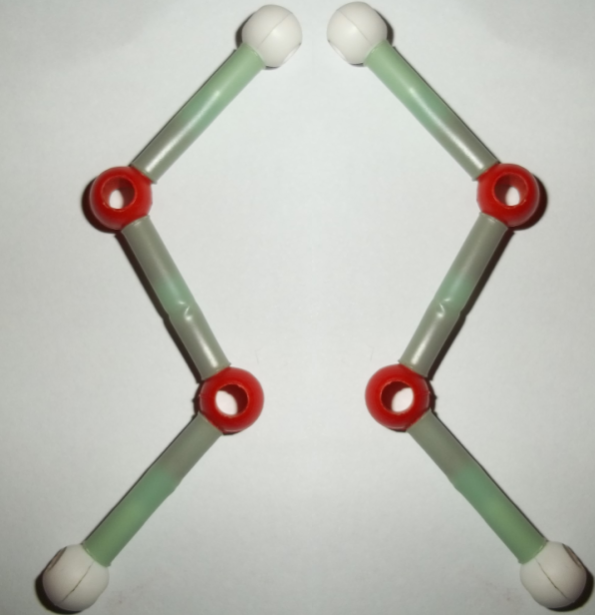
\includegraphics[width=.1\textwidth]{photos/H2O2_models.png} & 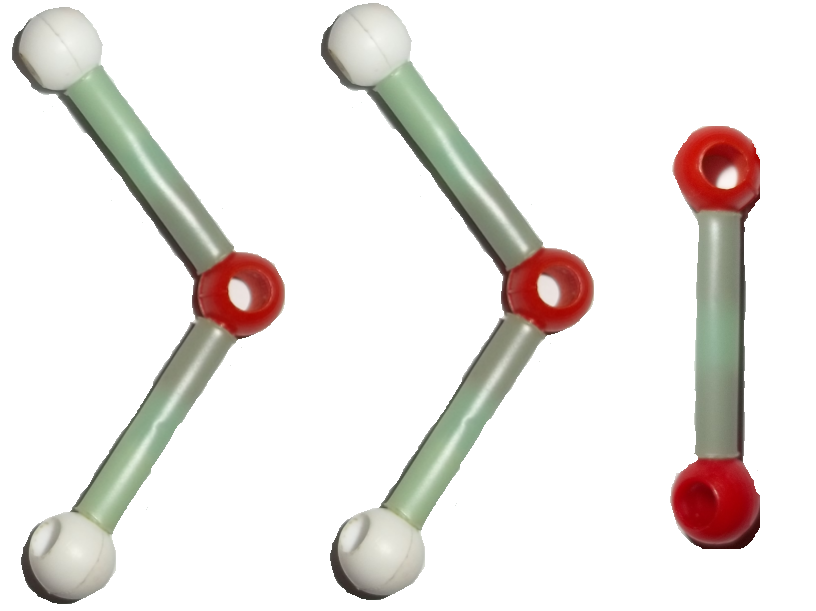
\includegraphics[width=.1\textwidth]{photos/H2O_O2.png} \\ \hline
   \textbf{Molecules} & two molecules & three molecules \\ \hline
\textbf{Energy changes} & energy taken in when bonds are broken & energy given off when bonds are formed \\ \hline
\textbf{Mass is conserved} & $4(1,01) + 4(16,0) = 68,04$ & $2(18,02) + 2(16,0) = 68,04$ \\ \hline
\textbf{Atoms are conserved} & 4 oxygen atoms, 4 hydrogen atoms & 4 oxygen atoms, 4 hydrogen atoms \\ \hline
  \end{tabular}
 \end{center}
\caption{Important concepts in chemical change}
\label{tab:chemchangeconcepts}
\end{table}
\begin{exercises}{Physical and chemical change}
 For each of the following say whether a chemical or a physical change occurs.
\begin{enumerate}[noitemsep, label=\textbf{\arabic*}. ]
\item Melting candle wax.
\item Mixing sodium chloride ($\text{NaCl}$) and silver nitrate ($\text{AgNO}_3$) to form silver chloride ($\text{AgCl}$).
\item Mixing hydrochloric acid ($\text{HCl}$) and magnesium ribbon ($\text{Mg}$) to form magnesium chloride ($\text{MgCl}_{2}$).
\item Dissolving salt in water.
\item Tearing a piece of magnesium ribbon. 
\end{enumerate}
\par \raisebox{-5 pt}{
\includegraphics[width=0.5cm]{col11305.imgs/summary_www.png}} Find the answers with the shortcodes:
 \par \begin{tabular}[h]{cccccc}
 (1.) l2z  &  u  &   &   &    &   & \end{tabular}
\end{exercises}

    \label{m38711*cid5}
            \section{Conservation of atoms and mass in reactions}
            \nopagebreak
      \label{m38711*id64489}In a chemical reaction the total mass of the all the substances taking part in the reaction remains the same. Also, the number of \textbf{atoms} in a reaction remains the same. Mass cannot be created or destroyed in a chemical reaction.\par 
\Definition{Law of conservation of mass}{The law of conservation of mass states that the total mass of substances taking part in a chemical reaction is conserved during the reaction.}
Table~\ref{tab:chemchangeconcepts} illustrates this law for the decomposition of hydrogen peroxide. The following activity allows you to see this for yourself using models.
            \begin{activity}{The conservation of atoms in chemical reactions }
            \nopagebreak
            \label{m38711*id64844}\noindent
\textbf{Materials:} \\ Coloured modelling clay rolled into balls or marbles and prestick to represent atoms. Each colour will represent a different element.
        \par 
      \label{m38711*id64882}\noindent
\textbf{Method:}\\
      \label{m38711*id64889}\begin{enumerate}[noitemsep, label=\textbf{\arabic*}. ] 
\label{m38711*uid36}\item Build your reactants. Use marbles and prestick or modelling clay to represent the reactants and put these on one side of your table. Make at least ten ($\text{H}_{2}$) units and at least five ($\text{O}_{2}$) units.
\label{m38711*uid37}\item Place the $\text{H}_{2}$ and $\text{O}_{2}$ units on a table. The table represents the 'test tube' where the reaction is going to take place. 
\label{m38711*uid38}\item Now count the number of atoms ($\text{H}$ and $\text{O}$) you have in your 'test tube'. Fill in the reactants column in the table below. Refer to table~\ref{tab:chemchangeconcepts} to help you fill in the mass row.
\label{m38711*uid39}\item Let the reaction take place. Each person can now take the $\text{H}$ and $\text{O}$ unit and use them to make water units. Break the $\text{H}$ and $\text{O}$ units apart and build $\text{H}_{2}\text{O}$ units with the parts. These are the products. Place the products on the table.
\item When the 'reaction' has finished (i.e. when all the $\text{H}$ and $\text{O}$ units have been used) count the number of atoms ($\text{H}$ and $\text{O}$) and complete the table.
\item What do you notice about the number of atoms for the reactants, compared to the products?
\item Write a balanced equation for this reaction and use your models to build this equation.
\end{enumerate}
        \par 
\begin{table}[H]
 \begin{center}
  \begin{tabular}{|l|l||l|} \hline
& \textbf{Reactants} & \textbf{Products} \\ 
& 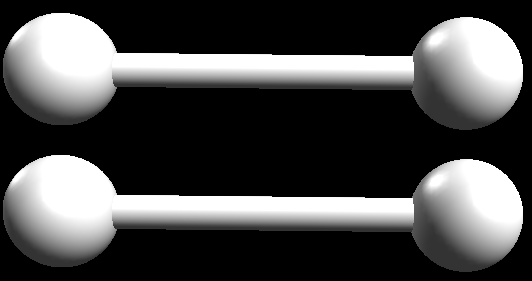
\includegraphics[width=.1\textwidth]{photos/hydrogen.png} 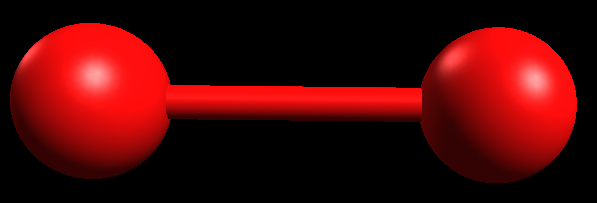
\includegraphics[width=.1\textwidth]{photos/oxygen.png} & \includegraphics[width=.1\textwidth]{photos/water.png} \\ \hline
   \textbf{Number of molecules} &  &  \\ \hline
\textbf{Mass} &  &  \\ \hline
\textbf{Number of atoms} &  &  \\ \hline
  \end{tabular}

 \end{center}

\end{table}

      \label{m38711*id65031}\noindent{}\textbf{Discussion}
     You should have noticed that the number of atoms in the reactants is the same as the number of atoms in the product. The number of atoms is conserved during the reaction. However, you will also see that the molecules in the reactants and products is not the same. The number of molecules is not conserved during the reaction.
 \par 
\end{activity}
\label{m38711*eip-14}
            \begin{i_experiment}{Conservation of matter}
            \nopagebreak
            \label{m38711*eip-453}\noindent{}\textbf{Aim:}
To prove the law of conservation of matter experimentally.
\par 
\label{m38711*eip792}\noindent{}\textbf{Materials:}
\textsl{Reaction 1:} \\
3 beakers; silver nitrate; sodium iodide; mass meter \\
\textsl{Reaction 2:} \\
 hydrochloric acid; bromothymol blue; sodium hydroxide solution; mass meter \\
 \textsl{Reaction 3:} \\
any effervescant tablet (e.g. Cal-C-Vita tablet), ballon; rubber band; mass meter; test tube; beaker
\par 
\label{m38711*eip-153}
\Warning{Always be careful when handling chemicals (particularly strong acids like hydrochloric acid) as you can burn yourself badly. }
	\par
      \label{m38711*id72432}\noindent
\textbf{Method:} \\
\begin{minipage}{.7\textwidth}
\textsl{Reaction 1} 
\label{m38711*id6342}\begin{enumerate}[noitemsep, label=\textbf{\arabic*}. ] 
            \item Solution 1: Dissolve $5~\text{g}$ of silver nitrate in $100~\text{ml}$ of water.
\item Solution 2: Dissolve $4.5~\text{g}$ of sodium iodide in $100~\text{ml}$ of water.
\item Determine the mass of the reactants.
\item Add solution 1 to solution 2. What do you observe? Has a chemical reaction taken place? 
\item Determine the mass of the products. 
\item What do you notice about the masses?
\item Write a balanced equation for this reaction.
\end{enumerate}
\end{minipage}
\begin{minipage}{.3\textwidth}
 \begin{center}
\scalebox{0.6}{
  \begin{pspicture}(0,0)(5,5)
\newpsstyle{white} {linestyle=solid,linewidth=.1,fillstyle=solid,fillcolor=white}
 \pstTubeEssais[etiquette,Numero={ $\text{AgNO}_{3}$},aspectLiquide1=white]
\pstTubeEssais[etiquette,Numero={ $\text{NaI}$},aspectLiquide1=white]  
  \end{pspicture}
}
 \end{center}
\end{minipage} \\
\begin{minipage}{.7\textwidth}
\textsl{Reaction 2:}
\label{m38711*id63452}\begin{enumerate}[noitemsep, label=\textbf{\arabic*}. ] 
\item Solution 1: Dissolve $0.4~\text{g}$ of sodium hydroxide in $100~\text{ml}$ of water. Add a few drops of bromothymol blue indicator to the solution. 
\item Solution 2: Measure $100~\text{ml}$ of $0,1~\text{M}$ hydrochloric acid solution into a beaker.
\item Determine the mass of the reactants.
\item Add small quantities of solution 2 to solution 1 (you can use a plastic pipette for this) until a colour change has taken place. Has a chemical reaction taken place?  
\item Determine the mass of hydrochloric acid added. (You do this by weighing the remaining solution, and subtracting this from the starting mass)
\item Compare the mass before the reaction to the total mass after the reaction. What do you notice?
\item Write a balanced equation for this reaction.
\end{enumerate}
\end{minipage}
\begin{minipage}{.3\textwidth}
 \begin{center}
\scalebox{.7}{
  \begin{pspicture}(0,0)(5,5)
\newpsstyle{white} {linestyle=solid,linewidth=.1,fillstyle=solid,fillcolor=white}
 \pstTubeEssais[etiquette,Numero={ $\text{NaOH}$},aspectLiquide1=white]
\pstTubeEssais[etiquette,Numero={ $\text{HCl}$},aspectLiquide1=white]    
  \end{pspicture}
}
 \end{center}
\end{minipage} \\
\begin{minipage}{.7\textwidth}
\textbf{Reaction 3}
\label{m38711*id634223}\begin{enumerate}[noitemsep, label=\textbf{\arabic*}. ] 
\item Half fill a large test tube with water.
\item Determine the mass of the test tube and water.
\item Break an effervescant tablet in two or three pieces and place them in a ballon.
\item Determine the mass of the ballon and tablet.
\item Fit the ballon tightly to the test tube, being careful to not drop the contents into the water. You can stand the test tube in a beaker to help you do this.
\item Determine the total mass of the test tube and ballon.
\item Lift the ballon so that the table goes into the water. What do you observe? Has a chemical reaction taken place?
\item Determine the mass of the test tube balloon combination.
\item What do you observe about the masses before and after the reaction?
\end{enumerate}
\end{minipage}
\begin{minipage}{.3\textwidth}
 \begin{center}
\scalebox{.6}{
  \begin{pspicture}(0,0)(5,5)
\newpsstyle{white} {linestyle=solid,linewidth=.1,fillstyle=solid,fillcolor=white}
 \pstTubeEssais[etiquette,Numero={ $\text{H}_{2}\text{O}$},aspectLiquide1=white]
   
  \end{pspicture}
}
 \end{center}
\end{minipage}
        \par \label{m38711*eip-768}\noindent{}\textbf{Results:}Fill in the following table for the total mass of reactants (starting materials) and products (ending materials).  \par 
    % \textbf{m38711*eip-581}\par
          \begin{table}[H]
    % \begin{table}[H]
    % \\ '' '0'
        \begin{center}
      \label{m38711*eip-581}
      \begin{tabular}{|l|l|l|l|}\hline
         &
        Reaction 1 &
        Reaction 2 &
        Reaction 3 \\ \hline
        Reactants &
         &
         &
        \\ \hline
        Products &
         &
         &
        \\ \hline
    \end{tabular}
      \end{center}
\end{table}
    \par
  \label{m38711*eip-634}Add the masses for the reactants for each reaction. Do the same for the products. For each reaction compare the mass of the reactants to the mass of the products. What do you notice? Is the mass conserved?\par \label{m38711*eip-65}In the experiment above you should have found that the total mass at the start of the reaction is the same as the mass at the end of the reaction. Mass does not appear or disappear in chemical reactions. Mass is conserved, in other words, the total mass you start with is the total mass you will end with.  \par
\end{i_experiment} 
\begin{exercises}{Conservation of atoms and mass} \noindent
Complete the following chemical reactions to show that atoms and mass are conserved. For each reaction give the total molecular mass of the reactants and the products.
 \begin{enumerate}[noitemsep, label=\textbf{\arabic*}.]
%Question 1
  \item Hydrogen gas combines with nitrogen gas to form ammonia.\\
\begin{figure}[H]
 \begin{center}
\scalebox{.5} % Change this value to rescale the drawing.
{
\begin{pspicture}(0,-2.01)(9.98,2.01)
\psframe[linewidth=0.04,dimen=outer](4.0,2.01)(0.0,-1.99)
\psframe[linewidth=0.04,dimen=outer](9.98,1.99)(5.98,-2.01)
\psline[linewidth=0.07cm,arrowsize=0.05291667cm 3.0,arrowlength=1.4,arrowinset=0.0]{->}(4.58,0.13)(5.42,0.13)
\pscircle[linewidth=0.04,dimen=outer](0.54,1.49){0.16}
\pscircle[linewidth=0.04,dimen=outer](0.84,1.49){0.16}
\rput{-46.441925}(1.196338,1.3458508){\pscircle[linewidth=0.04,dimen=outer](2.1666365,-0.7212986){0.16}}
\rput{-46.441925}(1.4181583,1.428068){\pscircle[linewidth=0.04,dimen=outer](2.3733635,-0.93870145){0.16}}
\rput{31.74865}(0.97520715,-1.4871812){\pscircle[linewidth=0.04,dimen=outer](3.1024454,0.97107095){0.16}}
\rput{31.74865}(1.0964445,-1.597797){\pscircle[linewidth=0.04,dimen=outer](3.3575547,1.1289291){0.16}}
\rput{80.2375}(1.1726402,-4.547286){\pscircle[linewidth=0.04,dimen=outer](3.2845652,-1.5778278){0.16}}
\rput{80.2375}(1.5062582,-4.351896){\pscircle[linewidth=0.04,dimen=outer](3.3354347,-1.2821721){0.16}}
\rput{38.670666}(-0.64319474,-0.8944015){\pscircle[linewidth=0.04,dimen=outer](0.9528874,-1.3637265){0.16}}
\rput{38.670666}(-0.47471237,-0.99965644){\pscircle[linewidth=0.04,dimen=outer](1.1871126,-1.1762736){0.16}}
\pscircle[linewidth=0.04,dimen=outer](0.52,-0.01){0.16}
\pscircle[linewidth=0.04,dimen=outer](0.82,-0.01){0.16}
\pscircle[linewidth=0.04,linecolor=blue,dimen=outer,fillstyle=solid,fillcolor=blue](1.39,0.88){0.25}
\pscircle[linewidth=0.04,linecolor=blue,dimen=outer,fillstyle=solid,fillcolor=blue](1.87,0.86){0.25}
\rput{47.621758}(0.82527715,-2.231293){\pscircle[linewidth=0.04,linecolor=blue,dimen=outer,fillstyle=solid,fillcolor=blue](2.9408476,-0.1805505){0.25}}
\rput{47.621758}(1.1875323,-2.370011){\pscircle[linewidth=0.04,linecolor=blue,dimen=outer,fillstyle=solid,fillcolor=blue](3.2791524,0.1605505){0.25}}
\end{pspicture}
} 
 \end{center}
\end{figure}
%Question 2
\item Hydrogen peroxide decomposes (breaks down) to form hydrogen and oxygen.\\
\begin{figure}[H]
 \begin{center}
\scalebox{.5} % Change this value to rescale the drawing.
{
\begin{pspicture}(0,-2.01)(9.98,2.01)
\psframe[linewidth=0.04,dimen=outer](4.0,2.01)(0.0,-1.99)
\psframe[linewidth=0.04,dimen=outer](9.98,1.99)(5.98,-2.01)
\psline[linewidth=0.07cm,arrowsize=0.05291667cm 3.0,arrowlength=1.4,arrowinset=0.0]{->}(4.58,0.13)(5.42,0.13)
\pscircle[linewidth=0.04,dimen=outer](0.62,1.39){0.16}
\pscircle[linewidth=0.04,linecolor=red,dimen=outer,fillstyle=solid,fillcolor=red](0.83,1.04){0.25}
\pscircle[linewidth=0.04,dimen=outer](1.54,0.69){0.16}
\pscircle[linewidth=0.04,linecolor=red,dimen=outer,fillstyle=solid,fillcolor=red](1.31,1.02){0.25}
\rput{-39.021122}(0.33611158,0.5916722){\pscircle[linewidth=0.04,dimen=outer](1.002982,-0.17846099){0.16}}
\rput{-39.021122}(0.57779634,0.46549466){\pscircle[linewidth=0.04,linecolor=red,dimen=outer,fillstyle=solid,fillcolor=red](0.9457715,-0.58259827){0.25}}
\rput{-39.021122}(1.1043428,0.513664){\pscircle[linewidth=0.04,dimen=outer](1.277018,-1.3015391){0.16}}
\rput{-39.021122}(0.8582375,0.6214732){\pscircle[linewidth=0.04,linecolor=red,dimen=outer,fillstyle=solid,fillcolor=red](1.3060981,-0.9003478){0.25}}
\rput{-93.27925}(2.4115129,4.595749){\pscircle[linewidth=0.04,dimen=outer](3.37574,1.159226){0.16}}
\rput{-93.27925}(2.218723,4.0344186){\pscircle[linewidth=0.04,linecolor=red,dimen=outer,fillstyle=solid,fillcolor=red](3.0143006,0.96959066){0.25}}
\rput{-93.27925}(2.4940598,2.916798){\pscircle[linewidth=0.04,dimen=outer](2.62426,0.28077406){0.16}}
\rput{-93.27925}(2.645873,3.4816551){\pscircle[linewidth=0.04,linecolor=red,dimen=outer,fillstyle=solid,fillcolor=red](2.9668763,0.49152064){0.25}}
\rput{62.03058}(0.100764476,-3.0118408){\pscircle[linewidth=0.04,dimen=outer](2.5551405,-1.4221209){0.16}}
\rput{62.03058}(0.33603603,-3.360519){\pscircle[linewidth=0.04,linecolor=red,dimen=outer,fillstyle=solid,fillcolor=red](2.96275,-1.4007995){0.25}}
\rput{62.03058}(1.0858464,-3.6818182){\pscircle[linewidth=0.04,dimen=outer](3.6048594,-0.937879){0.16}}
\rput{62.03058}(0.8310885,-3.354817){\pscircle[linewidth=0.04,linecolor=red,dimen=outer,fillstyle=solid,fillcolor=red](3.205534,-0.98624444){0.25}}
\end{pspicture} 
}
 \end{center}
\end{figure}
%Question 3
\item Calcium and oxygen gas react to form calcium oxide.\\
\begin{figure}[H]
 \begin{center}
\scalebox{.5} % Change this value to rescale the drawing.
{
\begin{pspicture}(0,-2.01)(9.98,2.01)
\definecolor{color314b}{rgb}{0.5019607843137255,0.0,1.0}
\psframe[linewidth=0.04,dimen=outer](4.0,2.01)(0.0,-1.99)
\psframe[linewidth=0.04,dimen=outer](9.98,1.99)(5.98,-2.01)
\psline[linewidth=0.07cm,arrowsize=0.05291667cm 3.0,arrowlength=1.4,arrowinset=0.0]{->}(4.58,0.13)(5.42,0.13)
\pscircle[linewidth=0.04,dimen=outer](0.54,1.49){0.16}
\pscircle[linewidth=0.04,dimen=outer](0.84,1.49){0.16}
\rput{38.670666}(0.8036014,-1.5376498){\pscircle[linewidth=0.04,dimen=outer](2.5928874,0.37627354){0.16}}
\rput{38.670666}(0.97208375,-1.6429048){\pscircle[linewidth=0.04,dimen=outer](2.8271127,0.5637264){0.16}}
\rput{112.262375}(0.40818247,-2.4516025){\pscircle[linewidth=0.04,dimen=outer](1.0268273,-1.0888188){0.16}}
\rput{112.262375}(0.5084122,-1.9635997){\pscircle[linewidth=0.04,dimen=outer](0.9131727,-0.8111812){0.16}}
\pscircle[linewidth=0.04,linecolor=color314b,dimen=outer,fillstyle=solid,fillcolor=color314b](1.61,1.16){0.25}
\pscircle[linewidth=0.04,linecolor=color314b,dimen=outer,fillstyle=solid,fillcolor=color314b](1.91,-0.26){0.25}
\pscircle[linewidth=0.04,linecolor=color314b,dimen=outer,fillstyle=solid,fillcolor=color314b](3.35,1.3){0.25}
\pscircle[linewidth=0.04,linecolor=color314b,dimen=outer,fillstyle=solid,fillcolor=color314b](0.49,0.06){0.25}
\pscircle[linewidth=0.04,linecolor=color314b,dimen=outer,fillstyle=solid,fillcolor=color314b](2.05,-1.42){0.25}
\pscircle[linewidth=0.04,linecolor=color314b,dimen=outer,fillstyle=solid,fillcolor=color314b](3.33,-0.94){0.25}
\end{pspicture} 
}
 \end{center}
\end{figure}
 \end{enumerate}
\par \raisebox{-5 pt}{
\includegraphics[width=0.5cm]{col11305.imgs/summary_www.png}} Find the answers with the shortcodes:
 \par \begin{tabular}[h]{cccccc}
 (1.) l2z  &  (2.) l2u  &  (3.) l2J  &    &    &   & \end{tabular}
\end{exercises}

    \label{m38711*cid6}
            \section{Law of constant composition}
            \nopagebreak
      \label{m38711*id65065}In any given chemical compound, the elements always combine in the same proportion with each other. This is the \textbf{law of constant proportion}.\par 
      \label{m38711*id65075}The \textbf{law of constant composition} says that, in any particular chemical compound, all samples of that compound will be made up of the same elements in the same proportion or ratio. For example, any water molecule is always made up of two hydrogen atoms and one oxygen atom in a 2:1 ratio. If we look at the relative masses of oxygen and hydrogen in a water molecule, we see that 94\% of the mass of a water molecule is accounted for by oxygen and the remaining 6\% is the mass of hydrogen. This mass proportion will be the same for any water molecule.\par 
      \label{m38711*id65089}This does not mean that hydrogen and oxygen always combine in a 2:1 ratio to form $\text{H}{}_{2}\text{O}$. Multiple proportions are possible. For example, hydrogen and oxygen may combine in different proportions to form $\text{H}{}_{2}\text{O}{}_{2}$ rather than $\text{H}{}_{2}\text{O}$. In $\text{H}{}_{2}\text{O}{}_{2}$, the H:O ratio is 1:1 and the mass ratio of hydrogen to oxygen is 1:16. This will be the same for any molecule of hydrogen peroxide.\par 
\begin{Investigation}{Law of constant composition}
 \textbf{Aim:} \\
To investigate the ratio in which compounds combine. \\
\textbf{Apparatus:} \\
\begin{minipage}{.4\textwidth}
\begin{itemize}[noitemsep]
\item $0,1~\text{M}$ silver nitrate ($\text{AgNO}_3$)
\item $0,1~\text{M}$ sodium chloride ($\text{NaCl}$)
\item $0,1~\text{M}$ lead nitrate ($\text{PbNO}_{3}$)
\item $0,1~\text{M}$ sodium iodide ($\text{NaI}$)
\item $0,1~\text{M}$ iron (III) chloride ($\text{FeCl}_{3}$)
\item $0,1~\text{M}$ sodium hydroxide ($\text{NaOH}$)
\item 9 large test tubes
\item 3 propettes
\end{itemize}
\end{minipage} 
\begin{minipage}{.6\textwidth}
 \begin{center}
\scalebox{.7}{
  \begin{pspicture}(0,0)(6,6)
\psset{unit=.5}
\newpsstyle{white} {linestyle=solid,linewidth=.1,fillstyle=solid,fillcolor=white}
% \newpsstyle{orange} {linestyle=solid,linewidth=.1,fillstyle=solid,fillcolor=white!20!orange}
%Silver nitrate
 \pstTubeEssais[aspectLiquide1=white,niveauLiquide1=30]
\pstTubeEssais[aspectLiquide1=white,niveauLiquide1=45] 
 \pstTubeEssais[aspectLiquide1=white,niveauLiquide1=60]
%Lead nitrate
% \pstTubeEssais[etiquette,Numero={$\text{PbNO}_{3}$},aspectLiquide1=white,niveauLiquide1=10]  
%  \pstTubeEssais[etiquette,Numero={$\text{PbNO}_{3}$},aspectLiquide1=white,niveauLiquide1=15]
% \pstTubeEssais[etiquette,Numero={$\text{PbNO}_{3}$},aspectLiquide1=white,niveauLiquide1=20]
% % Iron (III) chloride
%  \pstTubeEssais[etiquette,Numero={$\text{FeCl}_{3}$},aspectLiquide1=orange,niveauLiquide1=10]
% \pstTubeEssais[etiquette,Numero={$\text{FeCl}_{3}$},aspectLiquide1=orange,niveauLiquide1=15]  
%  \pstTubeEssais[etiquette,Numero={$\text{FeCl}_{3}$},aspectLiquide1=orange,niveauLiquide1=20] 
  \end{pspicture}
}
 \end{center}
\end{minipage}
\textbf{Method:}\\
\textsl{Reaction 1:} Prepare three test tubes with $5~\text{ml}$, $10~\text{ml}$ and $15~\text{ml}$  of silver nitrate respectively. Using a clean propette add $5~\text{ml}$ of sodium chloride to each one and observe what happens. Write a balanced equation for this reaction.\\
\textsl{Reaction 2:} Prepare three test tubes with $5~\text{ml}$, $10~\text{ml}$ and $15~\text{ml}$  of lead nitrate respectively. Using a clean propette add $5~\text{ml}$ of sodium iodide to each one and observe what happens. Write a balanced equation for this reaction.\\
\textsl{Reaction 3:} Prepare three test tubes with $5~\text{ml}$, $10~\text{ml}$ and $15~\text{ml}$  of sodium hydroxide respectively. Add $5~\text{ml}$ of iron(III) chloride to each one and observe what happens. Write a balanced equation for this reaction. \\
\textbf{Discussion and conclusion:} \\
For each of the three reactions you should have found that a reaction occurs (as seen by the presence of a precipitate) when the amount of the reactants is greater than or equal to the ratio in which the reactants combine.  
\end{Investigation}

    \label{m38711*cid7}
            \subsection*{Volume relationships in gases}
            \nopagebreak
      \label{m38711*id65179}In a chemical reaction between gases, the relative volumes of the gases in the reaction are present in a ratio of small whole numbers if all the gases are at the same temperature and pressure. This relationship is also known as \textbf{Gay-Lussac's Law}.\par 
      \label{m38711*id65189}For example, in the reaction between hydrogen and oxygen to produce water, two volumes of $\text{H}{}_{2}$ react with 1 volume of $\text{O}_{2}$ to produce 2 volumes of $\text{H}_{2}\text{O}$.\par 
      \label{m38711*id65237}$2\text{H}_{2}\text{(g)} +\text{O}_{2} \text{(g)} \to 2\text{H}_{2}\text{O} (\ell)$\par 
      \label{m38711*id65282}In the reaction to produce ammonia, one volume of nitrogen gas reacts with three volumes of hydrogen gas to produce two volumes of ammonia gas.\par 
      \label{m38711*id65286}$\text{N}_{2} \text{(g)}+3\text{H}_{2} \text{(g)} \to 2\text{NH}_{3} \text{(g)}$
      \par  
    \label{m38711*cid8}
            \section{Summary}
            \nopagebreak
\label{m38711*id972312}
The following video provides a summary of the concepts covered in this chapter.
    \setcounter{subfigure}{0}
	\begin{figure}[H] % horizontal\label{m38711*summary}
    \textnormal{Physical and chemical change} \nopagebreak
  \label{m38711*yt-media1}\label{m38711*yt-video1}
            \raisebox{-5 pt}{ 
\includegraphics[width=0.5cm]{col11305.imgs/summary_www.png}} { (Video:  P10058 )}
 \end{figure}       
\par  
      \label{m38711*id65342}\begin{enumerate}[noitemsep, label=\textbf{\arabic*}. ] 
            \label{m38711*uid40}\item Matter does not stay the same. It may undergo physical or chemical changes.
\label{m38711*uid41}\item A \textbf{physical change} means that the form of matter may change, but not its identity. For example, when water evaporates, the energy and the arrangement of water molecules will change, but not the structure of the water molecules themselves.
\label{m38711*uid42}\item During a physical change, the \textbf{arrangement of particles} may change but the mass, number of atoms and number of molecules will stay the same.
\label{m38711*uid43}\item Physical changes involve small changes in \textbf{energy} and are easily reversible.
\label{m38711*uid44}\item A chemical change occurs when one or more substances change into other materials. A chemical reaction involves the formation of new substances with \textbf{different properties}. For example, magnesium and oxygen react to form magnesium oxide ($\text{MgO}$) \label{m38711*uid45}\item A chemical change may involve a \textbf{decomposition} or \textbf{synthesis} reaction. During chemical change, the mass and number of atoms is conserved, but the number of molecules is not always the same.
\label{m38711*uid46}\item Chemical reactions involve large changes in energy. Chemical reactions are not easily reversible.
\label{m38711*uid48}\item The \textbf{law of conservation of mass} states that the total mass of all the substances taking part in a chemical reaction is conserved and the number of atoms of each element in the reaction does not change when a new product is formed.
\label{m38711*uid49}\item The \textbf{conservation of energy principle} states that energy cannot be created or destroyed, it can only change from one form to another.
\label{m38711*uid50}\item The \textbf{law of constant composition} states that in any particular compound, all samples of that compound will be made up of the same elements in the same proportion or ratio.
\label{m38711*uid51}\item \textbf{Gay-Lussac's Law} states that in a chemical reaction between gases, the relative volumes of the gases in the reaction are present in a ratio of small whole numbers if all the gases are at the same temperature and pressure.
\end{enumerate}
\label{m38711*secfhsst!!!underscore!!!id584}
            \begin{eocexercises}{Physical and chemical change}
            \nopagebreak \noindent
      \label{m38711*id65631}\begin{enumerate}[noitemsep, label=\textbf{\arabic*}. ] 
%Question 1
            \label{m38711*uid6234}\item For each of the following definitions give one word or term:
\label{m38711*id632243}\begin{enumerate}[noitemsep, label=\textbf{\alph*}. ] 
            \item A change that can be seen or felt, where the particles involved are not broken up in any way\item The formation of new substances in a chemical reaction\item A reaction where a new product is formed from elements or smaller compounds\end{enumerate}
%Question 2
\label{m38711*id63272}\item State the conservation of energy principle.
%Question 3
\label{m38711*id6244}\item Explain how a chemical change differs from a physical change.
%Question 4
\label{m38711*uid52}\item Complete the following table by saying whether each of the descriptions is an example of a physical or chemical change:
    % \textbf{m38711*id65648}\par
          \begin{table}[H]
    % \begin{table}[H]
    % \\ 'id2931526' '1'
        \begin{center}
      \label{m38711*id65648}
    \noindent
      \begin{tabular}{|l|l|}\hline
        \textbf{Description} &
        \textbf{Physical or chemical} \\ \hline
        hot and cold water mix together &
     \\ \hline
        milk turns sour &
     \\ \hline
        a car starts to rust &
       \\ \hline
        food digests in the stomach &
       \\ \hline
        alcohol disappears when it is placed on your skin &
       \\ \hline
        warming food in a microwave &
     \\ \hline
        separating sand and gravel &
       \\ \hline
        fireworks exploding &
       \\ \hline
    \end{tabular}
      \end{center}
\end{table}
    \par
%Question 5
          \label{m38711*uid53}\item For each of the following reactions, say whether it is an example of a synthesis or decomposition reaction:
\label{m38711*id65862}\begin{enumerate}[noitemsep, label=\textbf{\alph*}. ] 
            \label{m38711*uid54}\item 
$\left({\text{NH}}_{4}{\right)}_{2}{\text{CO}}_{3}\to {\text{NH}}_{3}+{\text{CO}}_{2}+\text{H}_{2}\text{O}$
\label{m38711*uid56}\item ${\text{N}}_{2}\left(\text{g}\right)+3{\text{H}}_{2}\left(\text{g}\right)\to 2{\text{NH}}_{3} \text{(g)}$\label{m38711*uid57}\item 
${\text{CaCO}}_{3} \to \text{CaO}+{\text{CO}}_{2}$\end{enumerate}
%Question 6
                \label{m38711*uid58}\item For the following equation:
${\text{CaCO}}_{3}\left(\text{s}\right)\to \text{CaO}+{\text{CO}}_{2}$
show that the 'law of conservation of mass' applies. Draw sub-microscopic diagrams to represent this reaction.\newline
        \end{enumerate}
  \label{m38711**end}
  \label{324e353f2415b0f24a8077f8f18039bb**end}
\par \raisebox{-5 pt}{
\includegraphics[width=0.5cm]{col11305.imgs/summary_www.png}} Find the answers with the shortcodes:
 \par \begin{tabular}[h]{cccccc}
 (1.) l2z  &  (2.) l2u  &  (3.) l2J  &  (4.) l3q  &  (5.) l3l  &  (6.) l3i  & \end{tabular}
\end{eocexercises}
